\documentclass{article}

% if you need to pass options to natbib, use, e.g.:
%     \PassOptionsToPackage{numbers, compress}{natbib}
% before loading neurips_2018

% ready for submission
% \usepackage{neurips_2018}

% to compile a preprint version, e.g., for submission to arXiv, add add the
% [preprint] option:
%     \usepackage[preprint]{neurips_2018}

% to compile a camera-ready version, add the [final] option, e.g.:
     \usepackage[final]{neurips_2018}

% to avoid loading the natbib package, add option nonatbib:
%     \usepackage[nonatbib]{neurips_2018}

\usepackage[utf8]{inputenc} % allow utf-8 input
\usepackage[T1]{fontenc}    % use 8-bit T1 fonts
\usepackage{hyperref}       % hyperlinks
\usepackage{url}            % simple URL typesetting
\usepackage{booktabs}       % professional-quality tables
\usepackage{amsfonts}       % blackboard math symbols
\usepackage{nicefrac}       % compact symbols for 1/2, etc.
\usepackage{microtype}      % microtypography

\title{Continual Learning on CLVision-Challenge}

% The \author macro works with any number of authors. There are two commands
% used to separate the names and addresses of multiple authors: \And and \AND.
%
% Using \And between authors leaves it to LaTeX to determine where to break the
% lines. Using \AND forces a line break at that point. So, if LaTeX puts 3 of 4
% authors names on the first line, and the last on the second line, try using
% \AND instead of \And before the third author name.

\author{%
  Haoran Zhu, Hua Sun \\
  Department of Electrical and Computer Engineering\\
  New York University\\
  \texttt{\{xxxxxx, hs4062\}@nyu.edu} \\
  % examples of more authors
  % \And
  % Coauthor \\
  % Affiliation \\
  % Address \\
  % \texttt{email} \\
  % \AND
  % Coauthor \\
  % Affiliation \\
  % Address \\
  % \texttt{email} \\
  % \And
  % Coauthor \\
  % Affiliation \\
  % Address \\
  % \texttt{email} \\
  % \And
  % Coauthor \\
  % Affiliation \\
  % Address \\
  % \texttt{email} \\
}

\begin{document}
% \nipsfinalcopy is no longer used

\maketitle

\begin{abstract}
  PlaceHolder
\end{abstract}

\section{Introduction}

\section{Related Work}
In real life, data is coming as streams of information, thus the agent should have the ability to learn tasks continuously. However, the current dominant paradigm for machine learning is to generate a model for each task. This paradigm is \textit{isolated learning}\cite{zhiyuan2017lml} since it does not consider any related information or previous learned knowledge and it is contrast to human learning process.

Continual Learning, also known as Lifelong Learning, is defined to be an algorithm which is capable of extracting knowledge from a continuous stream of data without forgetting the old knowledge, i.e. catastrophic forgetting\cite{thrun1995lifelong}, this phenomenon occurs because the weights trained for task A have been changed for task B. In \cite{parisi2019continual}, the author summarizes four major methods to prevent catastrophic forgetting: regularization methods, dynamic architectures, replay and complementary learning systems.  

Regularization methods\cite{li2017learning}\cite{kirkpatrick2017overcoming} are inspired by theoretical neuroscience models which show that the previous learning knowledge can be protected from forgetting through synapse with a cascade of states yielding different levels of plasticity. They provide a way to solve catastrophic forgetting, but they comprise additional loss for protecting consolidated knowledge, which may be a trade-off on the performance of old and new tasks.

Dynamic architectures methods \cite{rusu2016progressive}\cite{yoon2017lifelong} try to solve catastrophic forgetting by changing the model architecture when new information comes. This method prevents catastrophic forgetting but can rise the complexity of architectures with the growth of new tasks.

Complementary learning theory shows a computational framework of modeling memory by the interplay of mammalian hippocampus and neocortex. Several works have been developed through this theory\cite{Mo19CLS}. Inspired by the generative role of hippocampus for the replay of previous experiences, \cite{Shin19DeepGen} proposed a dual-model architecture to replay previous tasks. 

In general, continual learning is a open problem to be solved and many works can be done in this field
 
 
\section{Dataset and Experiment Design} \label{design}
In this section, we introduce the dataset \textit{CORe50} realeased by CVPR Workshop. Their dataset consist of three parts, and due to the constraint of time, we only consider the first two part of the three challenges. Then, we select two representative approaches for Continual Learning, EWC and Piggyback, and introduce the theorem and some core details about them.

\subsection{Dataset and Tasks}
\textit{CORe50} is a new dataset specially designed for \textit{(C)ontinual (O)bject (Re)cognition}. Unlike \textit{permuted MNIST}  where new tasks to learn are obtained by simply scrambling the pixel positions, \textit{CORe50} is much more complex and a real life dataset. Datasets such as \textit{ImageNet} and \textit{Pascal VOC} provide a good playground for image classification and detection, but they have been designed with “static” evaluation and lack of multiple views of the same objects taken into different sessions, \textit{CORe50} solves the above problems and meets the requirement for continuous learning scenarios on computer vision.

It consists 50 domestic objects belonging to 10 categories. The dataset is separated into 11 distinct sessions (8 indoors and 3 outdoors) with different background and lightning. For each session and for each object, a 15 seconds video (at 20 fps) has been recorded with a Kinect 2.0 sensor delivering 300 RGB-D frames. The whole dataset consists of 164,866 128 × 128 RGB-D images: 11 sessions x 50 objects x (∼300*) frames per session.  Three of the eleven sessions (\#3, \#7 and \#10) have been selected for test and the remaining 8 sessions are used for training. 

\begin{figure}[h]
  \centering
  \captionsetup{width=0.6\textwidth}
  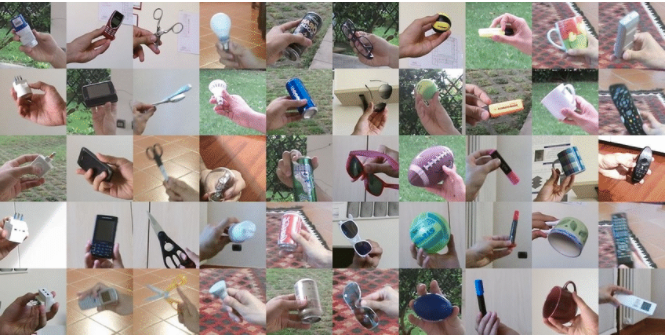
\includegraphics[width=0.8\textwidth]{figure/core50.png}
  \caption{Example images of the 50 objects in CORe50. Each column denotes one of the 10 categories.}
  \label{core50}
\end{figure}

There are three tasks in CVPR 2020 Workshop \textit{CLVision Challenge}:
\begin{itemize}
\item \textbf{New Classes(NC)}: New training patterns belonging to different classes become available in subsequent batches. In this case the model should be able to deal with the new classes without losing accuracy on the previous ones.
\item \textbf{New Instances(NI)}: New training patterns of the same classes become available in subse- quent batches with new poses and conditions (illumination, background, occlusion, etc.). A good model is expected to incrementally consolidate its knowledge about the known classes without compromising what it has learned before.
\item \textbf{New Instances and Classes(NIC)}: New training patterns belonging both to known and new classes become available in subsequent training batches. A good model is expected to consolidate its knowledge about the known classes and to learn the new ones.
\end{itemize} 

\subsection{EWC}
n brains, synaptic consolidation enables continual learning by reducing the plasticity of synapses that are vital to previously learned tasks.  \textit{EWC} is an algorithm that performs a similar operation in artificial neural networks by constraining important parameters to stay close to their old values. \textit{EWC} can be used in supervised learning and reinforcement learning problems to train several tasks sequentially without forgetting older ones.

\subsubsection{Theorem}
From a probabilistic perspective: optimizing the parameters is tantamount to finding their most probable values given some data D. We can compute this conditional probability $p(\theta | \mathcal{D})$ from the prior probability of the parameters $p(\theta)$ and the probability of the data $p(\mathcal{D}|\theta)$ by using Bayes’ rule:

\begin{equation}
\begin{aligned}
\log p(\theta | \mathcal{D})=\log p\left(\mathcal{D}_{B} | \theta\right)+\log p\left(\theta | \mathcal{D}_{A}\right)-\log p\left(\mathcal{D}_{B}\right)
\end{aligned}
\end{equation}

Similarly we can apply Bayes' rule on two continuous tasks A and B: 

\begin{equation}
\begin{aligned}
\log p(\theta | \mathcal{D})=\log p\left(\mathcal{D}_{B} | \theta\right)+\log p\left(\theta | \mathcal{D}_{A}\right)-\log p\left(\mathcal{D}_{B}\right)
\end{aligned}
\end{equation}

While $\log p(\mathcal{D}_{B}|\theta)$ is negative training loss for task B, we can optimize this by gradient descent.
$\log p(\mathcal{D}_{B})$ is a constant, we don't need to care about it when optimizing for the overall goal. $\log p(\theta|\mathcal{D}_{A})$ ‘s real value is intractable and will be approximated by Laplace approximation. The approximated value can further be the derivation regarding approximated mean value and its corresponding Hessian matrix. Noted that the expected value of Hessian matrix is the negative value of Fisher information matrix $F$, thus the original goal of maximizing $\log p(\theta | \mathcal{D})$ is equivalent to minimizing the following loss function:

\begin{equation}
\mathcal{L}(\theta)=\mathcal{L}_{B}(\theta)+\sum_{i} \frac{\lambda}{2} F_{i}\left(\theta_{i}-\theta_{A, i}^{*}\right)^{2}
\end{equation}

where $\mathcal{L}_{\mathcal{B}}(\theta)$ is the loss for task B only and hyperparameter $\lambda$ sets how important the old task is compared to the new task. When the third task comes, you can treat all previous tasks as the old task and repeat the above process. In the end, it can ensure the model can learn new tasks without changing the weights for the previous tasks too much. 





\subsection{Piggyback}
Piggyback is a upgrading version of Packnet, it uses pure mask layer to mask weights for new task. In this part, we introduce the core idea and the mathemetical representation of Piggyback. We also demonstrate some of the techniques used in training for Piggyback.

\subsubsection{Theorem}
\begin{figure}[h]
  \centering
  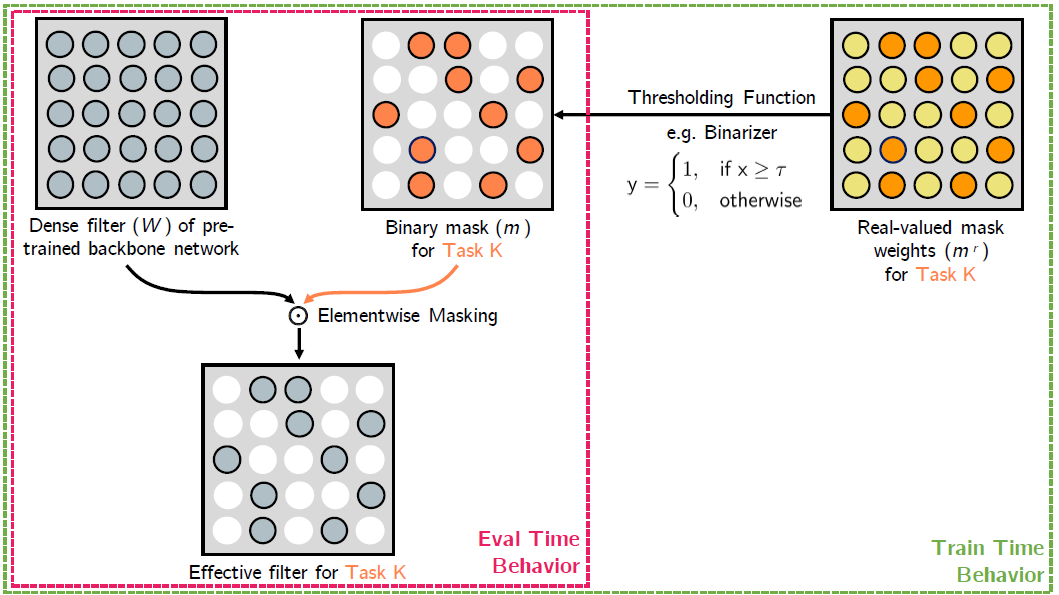
\includegraphics[width=0.8\textwidth]{figure/piggyback.png}
  \caption{Piggyback Overview}
  \label{piggy}
\end{figure}

Piggyback adopts masking weight for new task to overcome catastrophic forgetting. The core idea is to selectively mask the fixed weights of a base network, and then use this mask to predict the new task. That is, given model $\mathbf{W}$, whenever there is a new task streaming in, the model will initialize and optimize a binary value matrix $\mathbf{m}$, and use this mask to generate weight $\mathbf{W^\star}$ to be used in prediction for this specific new task. The gradient that backpropagates to the layer will not affect $\mathbf{W}$ but $\mathbf{m}$. In this way, for a given task, we can obtain filters that is consist of 0/1. For example, a dense weight vector [0.1, 0.2, 0.3, 0.4] could be filtered to [0, 0.2, 0.3, 0] after the binary masking. In short, we does not learn what are the `right` parameters but learn what is not the `right` parameters. Therefore, the choice of backbone network is crucial to the performance of piggyback because if the original weights are malfunctioning, pure masking cannot greatly improve the accuracy.

The structure of \textit{Piggyback} is shown in Figure \ref{piggy}. To explain the procedure for training, we consider an end to end fully-connected layer case. Denote $\mathbf{x}=[x_1, x_2, ..., x_m]$ as input, and $\mathbf{y}=[y_1, y_2, ..., y_n]$ as output. The weight matrix for this layer is $\mathbf{W}^{n\times m}$. Without loss of genrality, we can simply assume $\mathbf{y}=\mathbf{W}\mathbf{x}$ by ignoring the bias term. Suppose the loss function is $L$, the normal backpropagation equation for $\mathbf{W}$ is,
\begin{equation}
\centering
\begin{aligned}
\delta w_{ji}&=\frac{\partial L}{\partial w_{ji}} = (\frac{\partial L}{\partial y_j})\cdot (\frac{\partial y_j}{\partial w_{ji}}) \\
&= \delta y_j \cdot x_j \\
\therefore \delta \mathbf{W} &= \delta \mathbf{y} \cdot  \mathbf{x^T} \\
\end{aligned}
\end{equation}
In \textit{Piggyback}, the author has introduced a real value mask matrix $\mathbf{M_r}^{n\times m}$ and a manually set threshold $\tau$. $M_r$ is used to create the binary mask matrix $\mathbf{M}=[m_{ji}]$. We can obtain $m_{ji}$ by,
\begin{equation}
m_{ji}=\begin{cases}
1,\ \ &{\rm if}\ m^r_{ji}>\tau \\
0,\ \ &{\rm otherwise} \\
\end{cases}
\end{equation}
Then, for $y_j\in\mathbf{y}$, it gives $y_j=\sum_{i=1}^m w_{ji}\cdot m_{ji} \cdot x_i$. The backpropagation equation is used to update the real value matrix $M_r$. That is, during the whole training procedure, the weight matrix $\mathbf{W}$ is fixed as constant. In \textit{Piggyback}, the modified mask weigths updates as follows. Here, $A\odot B = C=[c_{ji}=A_{ji}B_{ji}]$. 

\begin{equation}
\begin{aligned}
\delta m_{ji}=\frac{\partial L}{\partial m_{ji}} &= (\frac{\partial L}{\partial y_j})\cdot (\frac{\partial y_j}{\partial m_{ji}}) \\
&= \delta y_j \cdot w_{ji} \cdot x_j \\
\therefore \delta \mathbf{m} &= (\delta \mathbf{y} \cdot x^T) \odot \mathbf{W} \\
\end{aligned}
\end{equation}
\subsubsection{Experiment Setting}
In practical, it is hard to derive the analytical solution to threshold $\tau$. In the original work, the author set $\tau=5e-3$. As for the matrix $\mathbf{m_r}$, the author initialized the value to 0.01. The best results are produced by Adam optimizer. In our experiment, we have inherited the parameter settings in the work. However, as mentioned in the previous statement, the crucial part for \textit{Piggyback} is that the base model have to be fine-tuned, otherwise the model will not work very well. We have also verified such phenomon in our experiment. To improve the performance, we modified the logic of the model. At the first task, we use the pure base model to perform the training, as the pre-trained network(ResNet50\cite{he2016deep}, in our case)cannot perform well on the given dataset. Then we begin performing mask and \textit{Piggyback}. This part will later be discussed in detail in Section \ref{eval}.






\section{Evaluation and Analyze}
\section{Conclusion}\label{conclusion}
In this project, we have looked thoroughly into the literature and legacy work of continual learning and then we choose two representative work, EWC and Piggyback, to experiment on the \textit{CLVision Challenge} issued by CVPR 2020 Workshop. For EWC, the performance is slightly improved compared to baseline model. For Piggyback, the initial performance is far worse even than baseline, then we propose a combination of EWC and Piggyback, which led to a much better performance in our project in both NI and NC cases. In the future, we could try out and continue to use and refine some dynamical approaches like DEN, and other incremental approaches\cite{zhou2012online}. 



\section{General formatting instructions}
\label{gen_inst}

The text must be confined within a rectangle 5.5~inches (33~picas) wide and
9~inches (54~picas) long. The left margin is 1.5~inch (9~picas).  Use 10~point
type with a vertical spacing (leading) of 11~points.  Times New Roman is the
preferred typeface throughout, and will be selected for you by default.
Paragraphs are separated by \nicefrac{1}{2}~line space (5.5 points), with no
indentation.

The paper title should be 17~point, initial caps/lower case, bold, centered
between two horizontal rules. The top rule should be 4~points thick and the
bottom rule should be 1~point thick. Allow \nicefrac{1}{4}~inch space above and
below the title to rules. All pages should start at 1~inch (6~picas) from the
top of the page.

For the final version, authors' names are set in boldface, and each name is
centered above the corresponding address. The lead author's name is to be listed
first (left-most), and the co-authors' names (if different address) are set to
follow. If there is only one co-author, list both author and co-author side by
side.

Please pay special attention to the instructions in Section \ref{others}
regarding figures, tables, acknowledgments, and references.

\section{Headings: first level}
\label{headings}

All headings should be lower case (except for first word and proper nouns),
flush left, and bold.

First-level headings should be in 12-point type.

\subsection{Headings: second level}

Second-level headings should be in 10-point type.

\subsubsection{Headings: third level}

Third-level headings should be in 10-point type.

\paragraph{Paragraphs}

There is also a \verb+\paragraph+ command available, which sets the heading in
bold, flush left, and inline with the text, with the heading followed by 1\,em
of space.

\section{Citations, figures, tables, references}
\label{others}

These instructions apply to everyone.

\subsection{Citations within the text}

The \verb+natbib+ package will be loaded for you by default.  Citations may be
author/year or numeric, as long as you maintain internal consistency.  As to the
format of the references themselves, any style is acceptable as long as it is
used consistently.

The documentation for \verb+natbib+ may be found at
\begin{center}
  \url{http://mirrors.ctan.org/macros/latex/contrib/natbib/natnotes.pdf}
\end{center}
Of note is the command \verb+\citet+, which produces citations appropriate for
use in inline text.  For example,
\begin{verbatim}
   \citet{hasselmo} investigated\dots
\end{verbatim}
produces
\begin{quote}
  Hasselmo, et al.\ (1995) investigated\dots
\end{quote}

If you wish to load the \verb+natbib+ package with options, you may add the
following before loading the \verb+neurips_2018+ package:
\begin{verbatim}
   \PassOptionsToPackage{options}{natbib}
\end{verbatim}

If \verb+natbib+ clashes with another package you load, you can add the optional
argument \verb+nonatbib+ when loading the style file:
\begin{verbatim}
   \usepackage[nonatbib]{neurips_2018}
\end{verbatim}

As submission is double blind, refer to your own published work in the third
person. That is, use ``In the previous work of Jones et al.\ [4],'' not ``In our
previous work [4].'' If you cite your other papers that are not widely available
(e.g., a journal paper under review), use anonymous author names in the
citation, e.g., an author of the form ``A.\ Anonymous.''

\subsection{Footnotes}

Footnotes should be used sparingly.  If you do require a footnote, indicate
footnotes with a number\footnote{Sample of the first footnote.} in the
text. Place the footnotes at the bottom of the page on which they appear.
Precede the footnote with a horizontal rule of 2~inches (12~picas).

Note that footnotes are properly typeset \emph{after} punctuation
marks.\footnote{As in this example.}

\subsection{Figures}

\begin{figure}
  \centering
  \fbox{\rule[-.5cm]{0cm}{4cm} \rule[-.5cm]{4cm}{0cm}}
  \caption{Sample figure caption.}
\end{figure}

All artwork must be neat, clean, and legible. Lines should be dark enough for
purposes of reproduction. The figure number and caption always appear after the
figure. Place one line space before the figure caption and one line space after
the figure. The figure caption should be lower case (except for first word and
proper nouns); figures are numbered consecutively.

You may use color figures.  However, it is best for the figure captions and the
paper body to be legible if the paper is printed in either black/white or in
color.

\subsection{Tables}

All tables must be centered, neat, clean and legible.  The table number and
title always appear before the table.  See Table~\ref{sample-table}.

Place one line space before the table title, one line space after the
table title, and one line space after the table. The table title must
be lower case (except for first word and proper nouns); tables are
numbered consecutively.

Note that publication-quality tables \emph{do not contain vertical rules.} We
strongly suggest the use of the \verb+booktabs+ package, which allows for
typesetting high-quality, professional tables:
\begin{center}
  \url{https://www.ctan.org/pkg/booktabs}
\end{center}
This package was used to typeset Table~\ref{sample-table}.

\begin{table}
  \caption{Sample table title}
  \label{sample-table}
  \centering
  \begin{tabular}{lll}
    \toprule
    \multicolumn{2}{c}{Part}                   \\
    \cmidrule(r){1-2}
    Name     & Description     & Size ($\mu$m) \\
    \midrule
    Dendrite & Input terminal  & $\sim$100     \\
    Axon     & Output terminal & $\sim$10      \\
    Soma     & Cell body       & up to $10^6$  \\
    \bottomrule
  \end{tabular}
\end{table}

\section{Final instructions}

Do not change any aspects of the formatting parameters in the style files.  In
particular, do not modify the width or length of the rectangle the text should
fit into, and do not change font sizes (except perhaps in the
\textbf{References} section; see below). Please note that pages should be
numbered.

\section{Preparing PDF files}

Please prepare submission files with paper size ``US Letter,'' and not, for
example, ``A4.''

Fonts were the main cause of problems in the past years. Your PDF file must only
contain Type 1 or Embedded TrueType fonts. Here are a few instructions to
achieve this.

\begin{itemize}

\item You should directly generate PDF files using \verb+pdflatex+.

\item You can check which fonts a PDF files uses.  In Acrobat Reader, select the
  menu Files$>$Document Properties$>$Fonts and select Show All Fonts. You can
  also use the program \verb+pdffonts+ which comes with \verb+xpdf+ and is
  available out-of-the-box on most Linux machines.

\item The IEEE has recommendations for generating PDF files whose fonts are also
  acceptable for NeurIPS. Please see
  \url{http://www.emfield.org/icuwb2010/downloads/IEEE-PDF-SpecV32.pdf}

\item \verb+xfig+ "patterned" shapes are implemented with bitmap fonts.  Use
  "solid" shapes instead.

\item The \verb+\bbold+ package almost always uses bitmap fonts.  You should use
  the equivalent AMS Fonts:
\begin{verbatim}
   \usepackage{amsfonts}
\end{verbatim}
followed by, e.g., \verb+\mathbb{R}+, \verb+\mathbb{N}+, or \verb+\mathbb{C}+
for $\mathbb{R}$, $\mathbb{N}$ or $\mathbb{C}$.  You can also use the following
workaround for reals, natural and complex:
\begin{verbatim}
   \newcommand{\RR}{I\!\!R} %real numbers
   \newcommand{\Nat}{I\!\!N} %natural numbers
   \newcommand{\CC}{I\!\!\!\!C} %complex numbers
\end{verbatim}
Note that \verb+amsfonts+ is automatically loaded by the \verb+amssymb+ package.

\end{itemize}

If your file contains type 3 fonts or non embedded TrueType fonts, we will ask
you to fix it.

\subsection{Margins in \LaTeX{}}

Most of the margin problems come from figures positioned by hand using
\verb+\special+ or other commands. We suggest using the command
\verb+\includegraphics+ from the \verb+graphicx+ package. Always specify the
figure width as a multiple of the line width as in the example below:
\begin{verbatim}
   \usepackage[pdftex]{graphicx} ...
   \includegraphics[width=0.8\linewidth]{myfile.pdf}
\end{verbatim}
See Section 4.4 in the graphics bundle documentation
(\url{http://mirrors.ctan.org/macros/latex/required/graphics/grfguide.pdf})

A number of width problems arise when \LaTeX{} cannot properly hyphenate a
line. Please give LaTeX hyphenation hints using the \verb+\-+ command when
necessary.

\subsubsection*{Acknowledgments}

Use unnumbered third level headings for the acknowledgments. All acknowledgments
go at the end of the paper. Do not include acknowledgments in the anonymized
submission, only in the final paper.

\section*{References}

References follow the acknowledgments. Use unnumbered first-level heading for
the references. Any choice of citation style is acceptable as long as you are
consistent. It is permissible to reduce the font size to \verb+small+ (9 point)
when listing the references. {\bf Remember that you can use more than eight
  pages as long as the additional pages contain \emph{only} cited references.}
\medskip

\small

[1] Alexander, J.A.\ \& Mozer, M.C.\ (1995) Template-based algorithms for
connectionist rule extraction. In G.\ Tesauro, D.S.\ Touretzky and T.K.\ Leen
(eds.), {\it Advances in Neural Information Processing Systems 7},
pp.\ 609--616. Cambridge, MA: MIT Press.

[2] Bower, J.M.\ \& Beeman, D.\ (1995) {\it The Book of GENESIS: Exploring
  Realistic Neural Models with the GEneral NEural SImulation System.}  New York:
TELOS/Springer--Verlag.

[3] Hasselmo, M.E., Schnell, E.\ \& Barkai, E.\ (1995) Dynamics of learning and
recall at excitatory recurrent synapses and cholinergic modulation in rat
hippocampal region CA3. {\it Journal of Neuroscience} {\bf 15}(7):5249-5262.

\end{document}